\section{Qualitative Analysis}
Based on the t-SNE results of the 5 composers in the Baroque period, the researchers noticed that the points are not that scattered and forms an arc like shape. Each composer in the Baroque period have points that are located near each other especially Boyce and Sammartini. The other 3 composers in the Baroque period are parts of the pattern that the Boyce and Sammartini produced.  This result may suggest that composers in the Baroque period have similar styles of composition. In the graph of the 5 Classical composers, the points also form a similar pattern except for 1 composer, Haydn. The consistency and the solidness of the points are more noticeable in the Classical period compared to the Baroque Period. In the 19th Century Period, the results are a bit scattered throughout the map and composers Clementi and Gossec are noticeably having their own pattern. The other 3 composers of the 19th Century are the ones that created a similar pattern. This results in the 19th Century suggests that composers during this time have their own style of compositions, within the 5 composers of the 19th Century. In the Romantic Period, the graph resulted in a more diverse pattern of each composers compared to the 19th Century. There is no specific pattern or style that was shown in the graph that could determine the style of the Romantic Period composers. The same goes with the 20th Century, various styles are shown in the graph. In the earlier Periods like Baroque and Classical, more consistent and similar pattern styles are observable. This analysis suggests that early composers tend to have similar styles in composing symphonies. Through time, composers in the 19th Century, Romantic, and 20th Century period are more unique in terms of the way they compose their symphonies.

In terms of transition, the researchers noticed that the most number of similar graphs, visually looking, are present in all periods but are more dominant in the periods of Classical, 19th and 20th Century Composers. An example is the compositions of Mozart, wherein his graph has a similar pattern with 19th Century composers Beethoven, Kalliwoda and Rubinstein. This pattern continues to be present in the works of the Romantic period composers Mendelssohn and a little bit of Tchaikovsky. Lastly, the trend continues in the 20th Century composers Rachmaninoff and Rubbra. The pattern described throughout the periods is observed as a round shape style. Shown below is the development of the pattern that rooted in the composition of Mozart.

\begin{figure}[h]
\caption{Classical: Mozart}
\centering
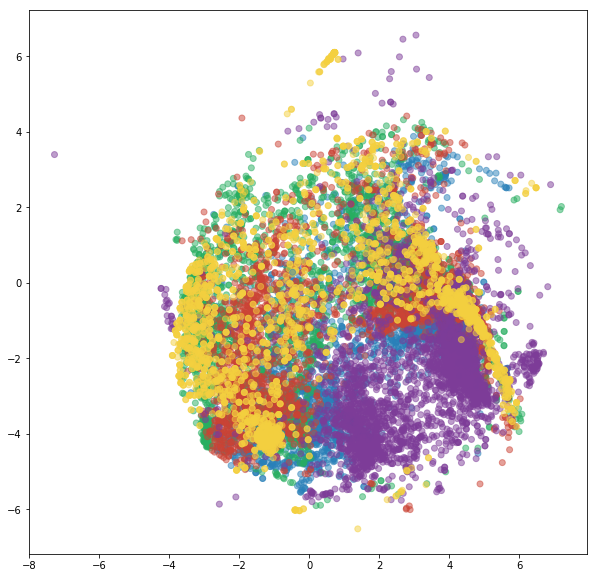
\includegraphics[scale=0.15]{P2C4}
\end{figure}

\begin{figure}[h]
\begin{minipage}{.5\textwidth}
  \captionof{figure}{19th Century: Kalliwoda}
  \centering
  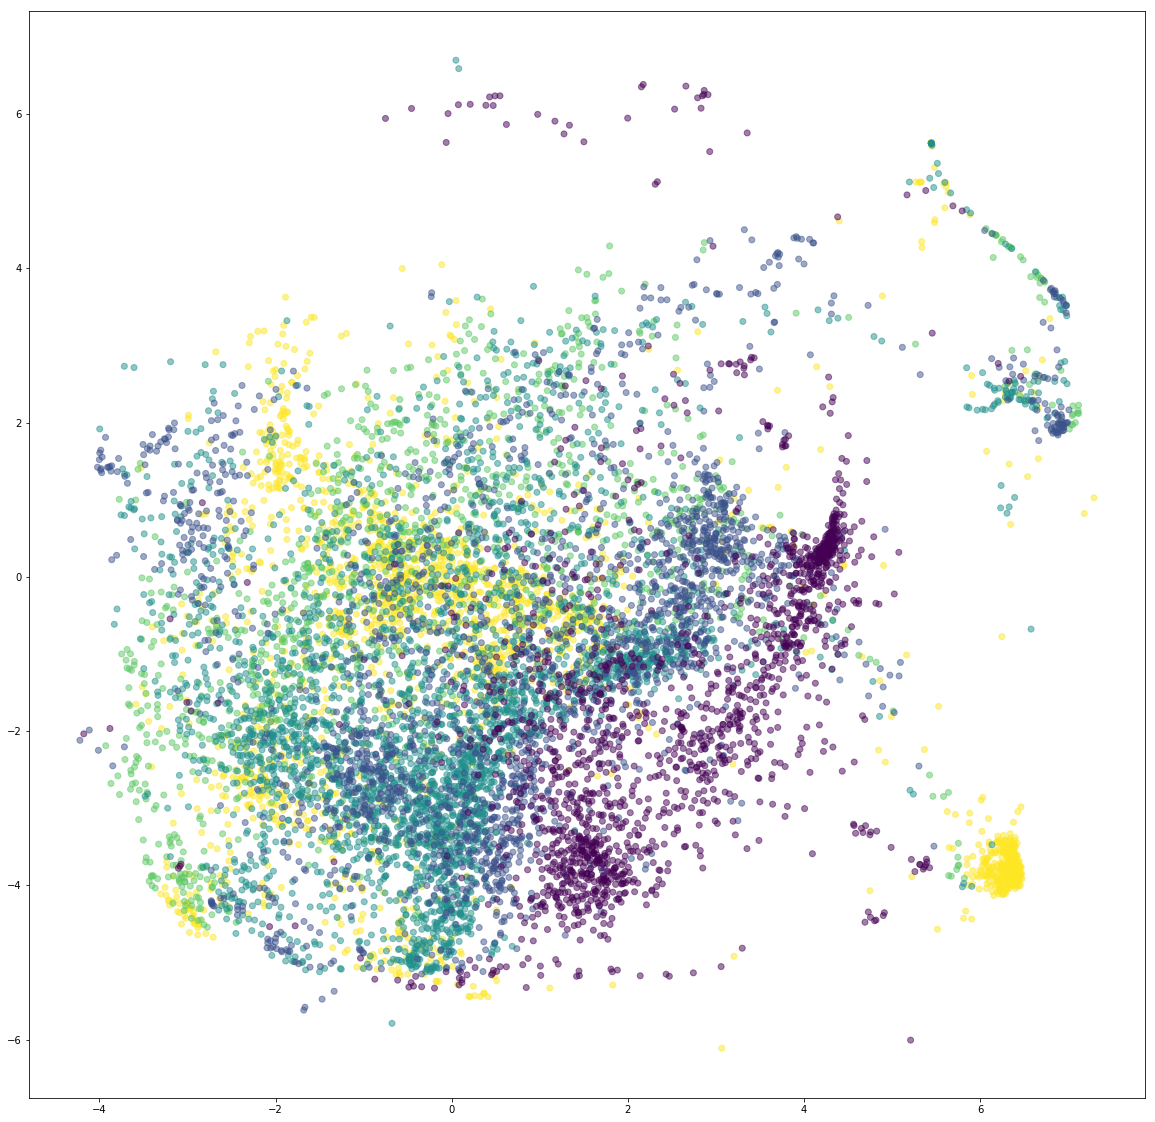
\includegraphics[scale=0.15]{P3C4}
  \label{fig:test2}
\end{minipage}
\begin{minipage}{.5\textwidth}
  \captionof{figure}{19th Century: Beethoven}
  \centering
  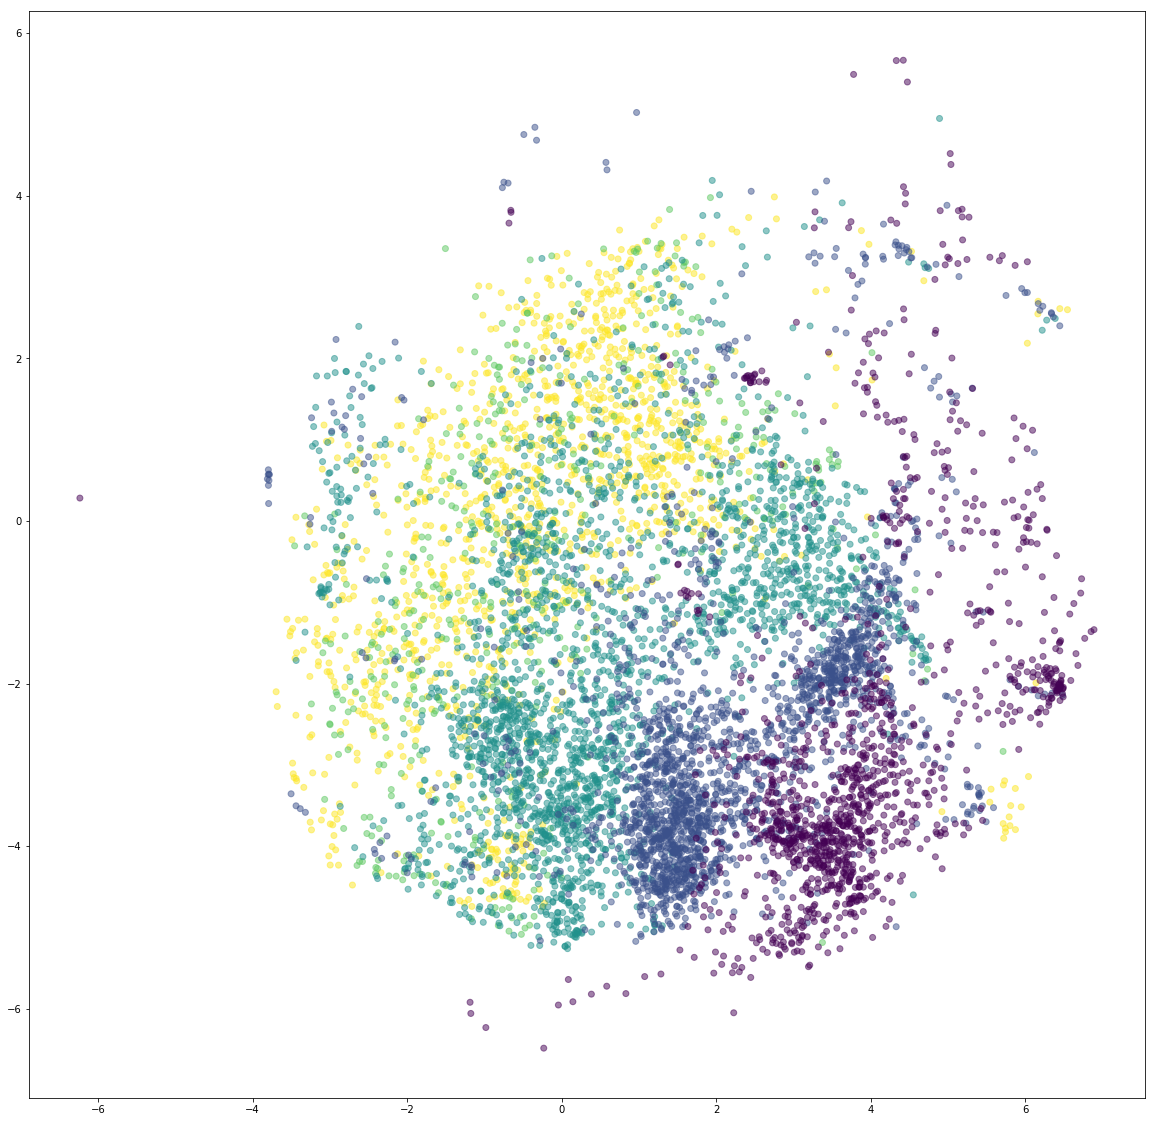
\includegraphics[scale=0.15]{P3C1}
  \label{fig:test1}
\end{minipage}
\end{figure}

\begin{figure}[h]
\begin{minipage}{.5\textwidth}
  \captionof{figure}{Romantic: Mendelssohn}
  \centering
  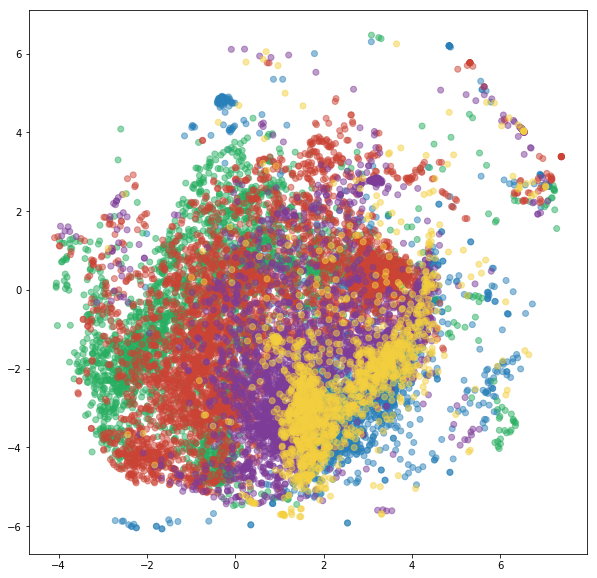
\includegraphics[scale=0.15]{P4C2}
  \label{fig:test2}
\end{minipage}
\begin{minipage}{.5\textwidth}
\caption{Romantic: Tchaikovsky}
\centering
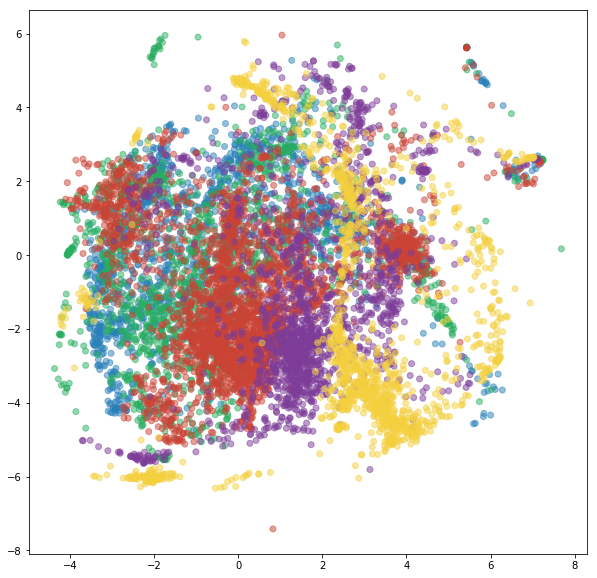
\includegraphics[scale=0.15]{P4C5}
 \label{fig:test3}
\end{minipage}
\end{figure}

\begin{figure}[h]
\begin{minipage}{.5\textwidth}
  \captionof{figure}{20th Cen: Rachmaninoff}
  \centering
  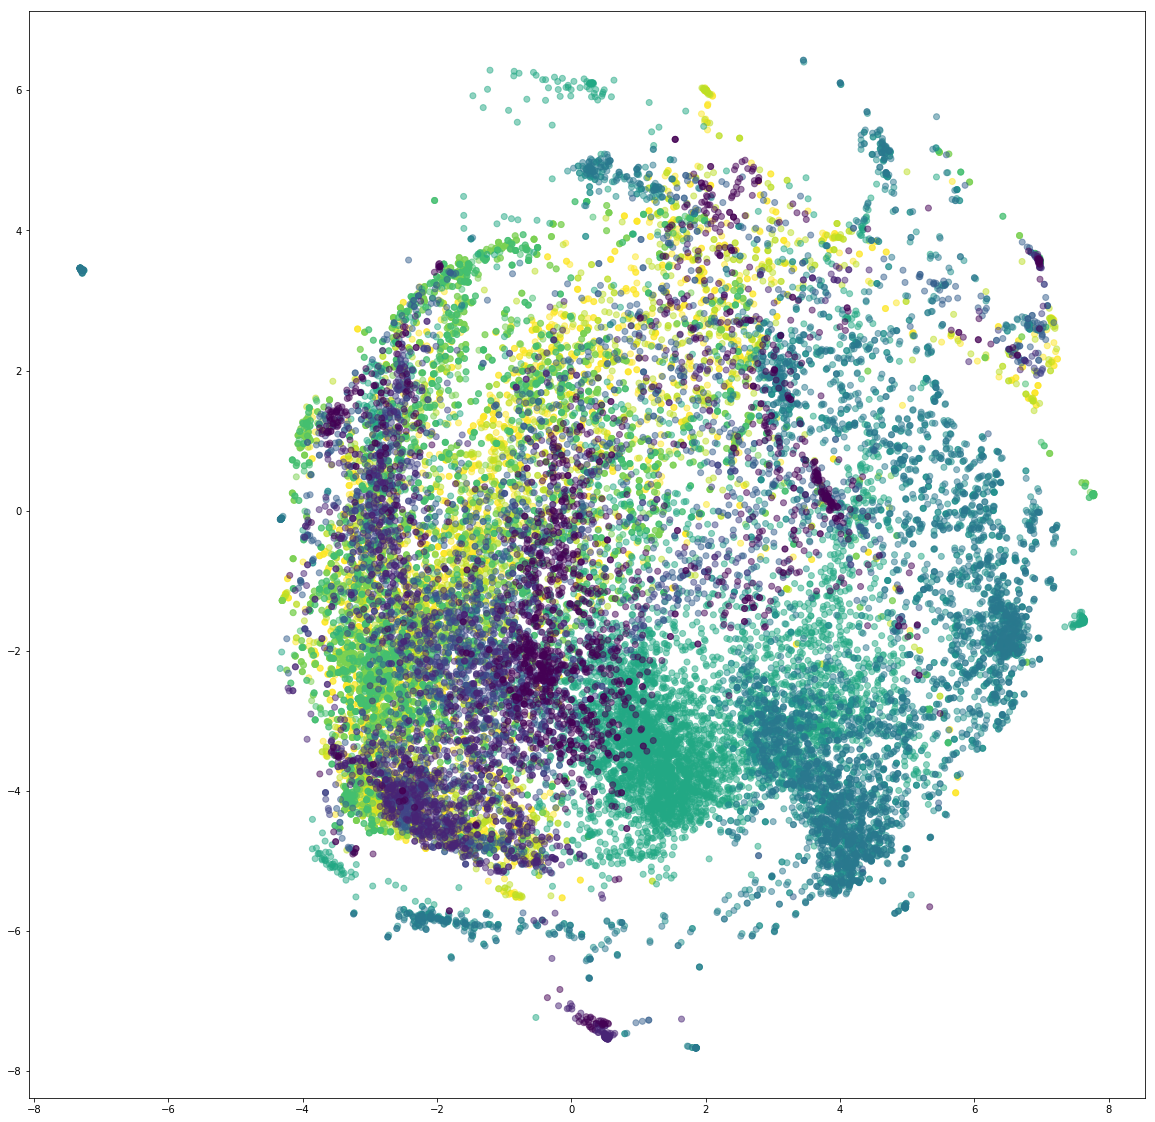
\includegraphics[scale=0.15]{P5C2}
  \label{fig:test2}
\end{minipage}
\begin{minipage}{.5\textwidth}
  \captionof{figure}{20th Cen: Rubbra}
  \centering
  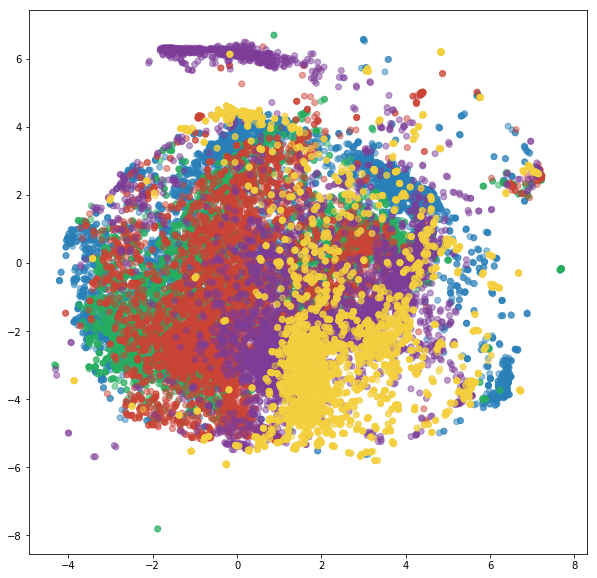
\includegraphics[scale=0.15]{P5C3}
  \label{fig:test1}
\end{minipage}
\end{figure}

\begin{figure}[h]
\caption{19th Century: Rubinstein}
\centering
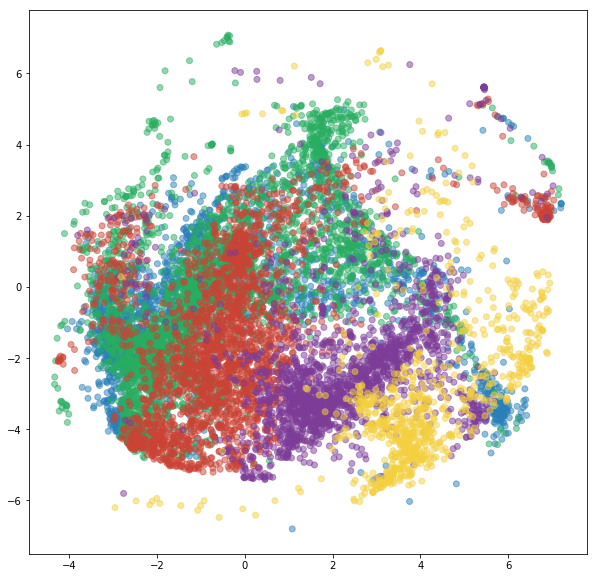
\includegraphics[scale=0.15]{P3C5}
\end{figure}